\documentclass[11pt,a4paper]{ltjsarticle}
\usepackage{amsmath,amssymb}
\usepackage{graphicx}
\usepackage{booktabs}
\usepackage{array}
\usepackage{float}
\usepackage{listings}
\usepackage{luatexja-fontspec}
\setmainjfont{HaranoAjiMincho-Regular}
\setsansjfont{HaranoAjiGothic-Medium}
\linespread{1.05}\selectfont

\lstset{
  basicstyle=\ttfamily\scriptsize,
  breaklines=true,
  columns=fullflexible,
  frame=single,
  keepspaces=true,
  numbers=left,
  numberstyle=\tiny,
  xleftmargin=2em
}

\begin{document}

\begin{center}
{\LARGE \textbf{視覚メディア処理I 第3回レポート}}
\end{center}
\vspace{1em}

\begin{flushright}
提出日: \today \\
学籍番号: 2611193 \\
氏名: 中井 平蔵
\end{flushright}

\section*{1. 使用画像と設定}

15枚の画像を、枚数の異なる4種類のセットに分けた。
分割方法を表1に、使用画像を図1に示す。

\begin{table}[H]
\centering
\caption{データセットの分割方法}
\begin{tabular}{lll}
\toprule
セット & 枚数 & 使用画像 \\
\midrule
\texttt{Set\_A\_3}  & 3  & \texttt{0.jpg}--\texttt{2.jpg} \\
\texttt{Set\_B\_7}  & 7  & \texttt{0.jpg}--\texttt{6.jpg} \\
\texttt{Set\_C\_11} & 11 & \texttt{0.jpg}--\texttt{10.jpg} \\
\texttt{Set\_D\_15} & 15 & \texttt{0.jpg}--\texttt{14.jpg} \\
\bottomrule
\end{tabular}
\end{table}

\begin{figure}[H]
\centering
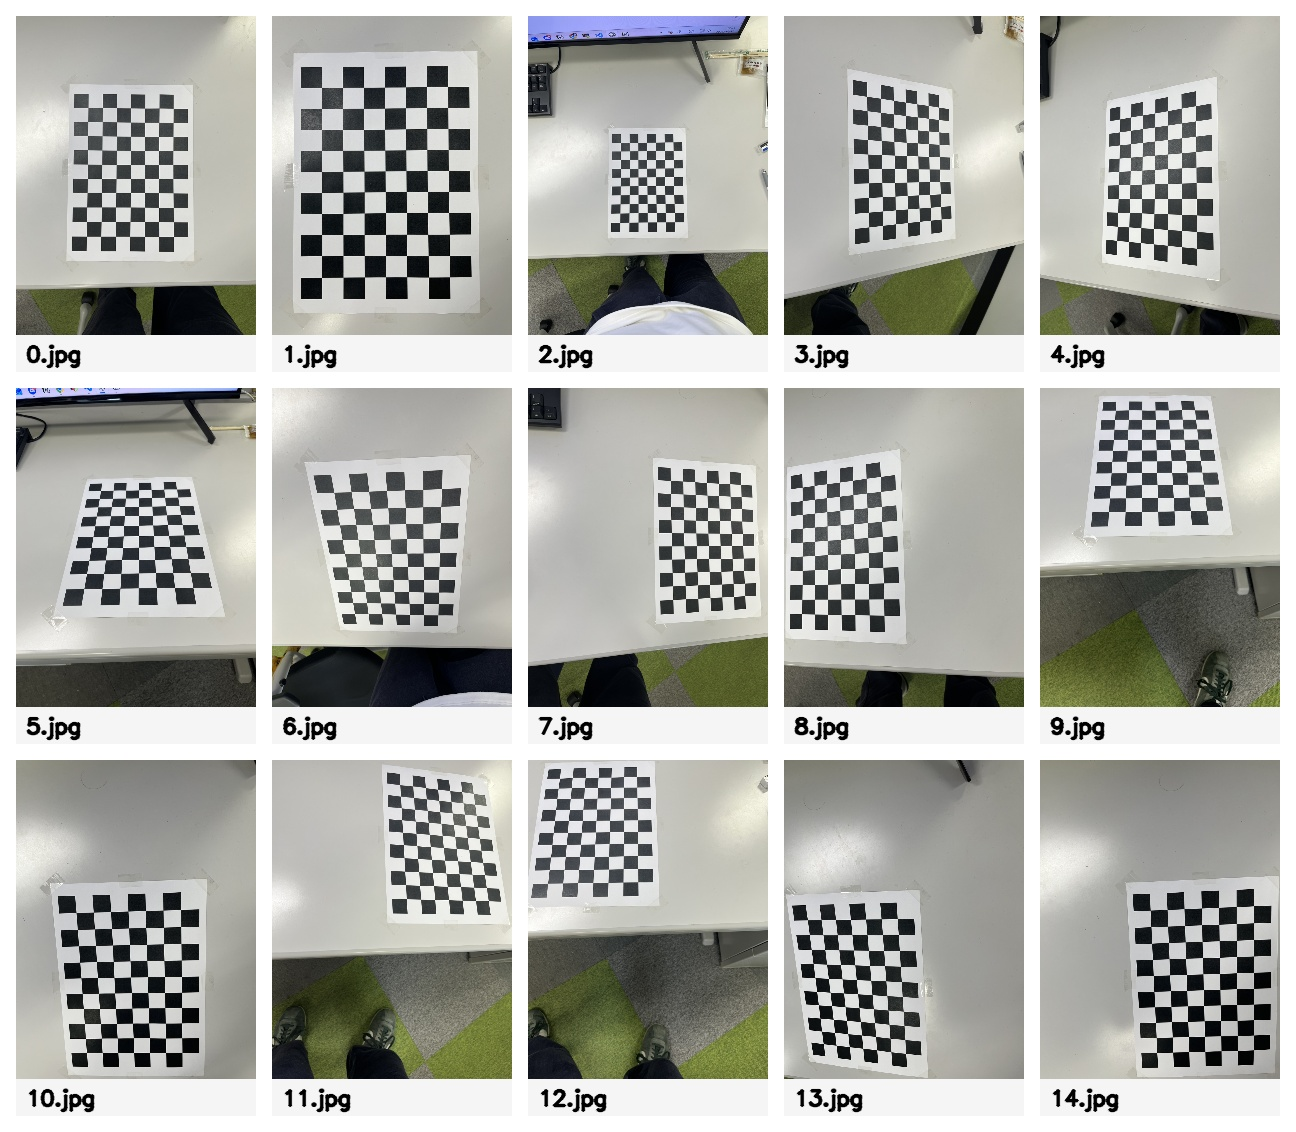
\includegraphics[width=0.82\linewidth]{calibration_outputs/dataset_overviews/Set_D_15_overview.jpg}
\caption{使用した15枚のキャリブレーション画像}
\end{figure}

各画像では、OpenCV によりチェッカーボードの内側交点を検出した。
今回使用したチェッカーボードは、横方向7点、縦方向10点の内側交点を持つため、
検出パターンサイズを
\[
(7,10)
\]
とした。1マスの実寸は \textbf{24 mm} として設定した。したがって、チェッカーボード平面上の
3次元点は、左上の内側交点を原点として
\[
\mathbf{X}_{ij} = (24i,\,24j,\,0)^\top\ \mathrm{[mm]}
\]
とした。ただし、$i=0,\ldots,6$、$j=0,\ldots,9$ である。

キャリブレーションの実装には OpenCV を用いた。チェッカーボード交点の検出には
\texttt{cv2.findChessboardCornersSB} を使用し、内部パラメータ推定には
\texttt{cv2.calibrateCamera} を使用した。

\section*{2. カメラモデル}

カメラの内部パラメータ行列を
\[
K =
\begin{bmatrix}
f_x & 0 & c_x \\
0 & f_y & c_y \\
0 & 0 & 1
\end{bmatrix}
\]
とする。ここで、$f_x,f_y$ はピクセル単位の焦点距離、
$c_x,c_y$ は主点座標である。

歪み係数は OpenCV の標準的なモデルに従い、
\[
(k_1,k_2,p_1,p_2,k_3)
\]
として推定した。$k_1,k_2,k_3$ は半径方向歪み、$p_1,p_2$ は接線方向歪みを表す。

再投影誤差は、画像から検出した交点 $\mathbf{x}_i$ と、推定したカメラパラメータで
3次元点を画像上に投影した点 $\hat{\mathbf{x}}_i$ の距離である。RMS誤差は
\[
\mathrm{RMS}
=
\sqrt{
\frac{1}{N}
\sum_{i=1}^{N}
\left\|
\mathbf{x}_i-\hat{\mathbf{x}}_i
\right\|^2
}
\]
で計算される。単位はピクセルであり、小さいほど検出点と再投影点の差が小さいことを示す。

\section*{3. 実行結果}

各セットで得られた内部パラメータと再投影誤差を表2に示す。
\texttt{OpenCV RMS} は \texttt{cv2.calibrateCamera} が返す全体のRMS再投影誤差である。
\texttt{Mean image RMS} は、各画像ごとに計算したRMS誤差の平均である。

\begin{table}[H]
\centering
\caption{画像セットごとの内部パラメータと再投影誤差}
\small
\begin{tabular}{lrrrrrr}
\toprule
セット & 枚数 & OpenCV RMS & Mean image RMS & $f_x$ & $f_y$ & $(c_x,c_y)$ \\
\midrule
\texttt{Set\_A\_3}  & 3  & 0.218 & 0.202 & 1235.763 & 1234.375 & (558.250, 727.926) \\
\texttt{Set\_B\_7}  & 7  & 0.295 & 0.283 & 1141.844 & 1140.028 & (566.494, 732.188) \\
\texttt{Set\_C\_11} & 11 & 0.344 & 0.331 & 1143.386 & 1141.363 & (562.532, 735.351) \\
\texttt{Set\_D\_15} & 15 & 0.425 & 0.416 & 1146.044 & 1143.997 & (560.469, 731.875) \\
\bottomrule
\end{tabular}
\end{table}

歪み係数を表3に示す。

\begin{table}[H]
\centering
\caption{画像セットごとの歪み係数}
\small
\begin{tabular}{lrrrrr}
\toprule
セット & $k_1$ & $k_2$ & $p_1$ & $p_2$ & $k_3$ \\
\midrule
\texttt{Set\_A\_3}  & 0.265 & -1.831 & $-3.67\times10^{-4}$ & $5.29\times10^{-4}$ & 4.219 \\
\texttt{Set\_B\_7}  & 0.233 & -1.350 & $-3.86\times10^{-4}$ & $3.66\times10^{-4}$ & 2.609 \\
\texttt{Set\_C\_11} & 0.181 & -0.883 & $4.96\times10^{-4}$ & $-6.25\times10^{-4}$ & 1.528 \\
\texttt{Set\_D\_15} & 0.098 & -0.260 & $-8.26\times10^{-4}$ & $-8.63\times10^{-4}$ & 0.274 \\
\bottomrule
\end{tabular}
\end{table}

各画像における最大の画像別RMS誤差は、\texttt{Set\_A\_3} で0.311 px、
\texttt{Set\_B\_7} で0.355 px、\texttt{Set\_C\_11} で0.508 px、
\texttt{Set\_D\_15} で0.533 pxであった。すべて1ピクセル未満であり、
検出した交点と再投影点のずれは小さい。

\section*{4. 再投影誤差の可視化}

再投影誤差が画像上でどの程度ずれているかを確認するため、検出点と再投影点を
同じ画像上に描画した。緑の点がOpenCVで検出した交点、赤の点が推定パラメータにより
再投影された点である。

\begin{figure}[H]
\centering
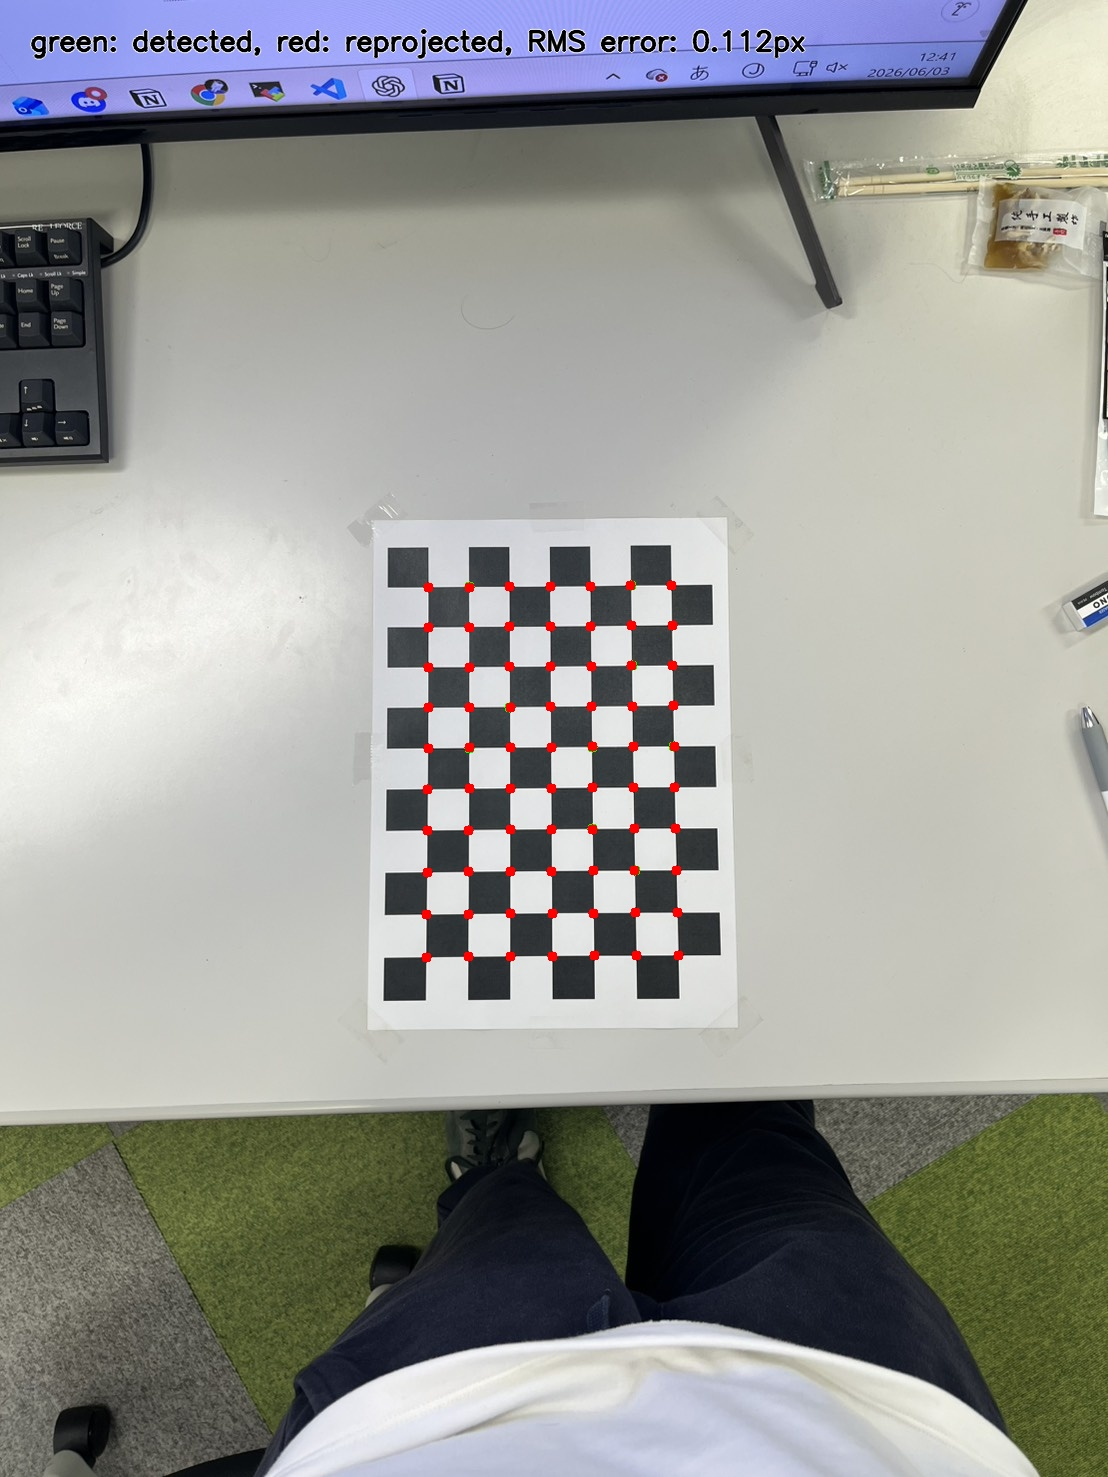
\includegraphics[width=0.46\linewidth]{calibration_outputs/Set_A_3/reprojection_plots/2_reprojection.jpg}
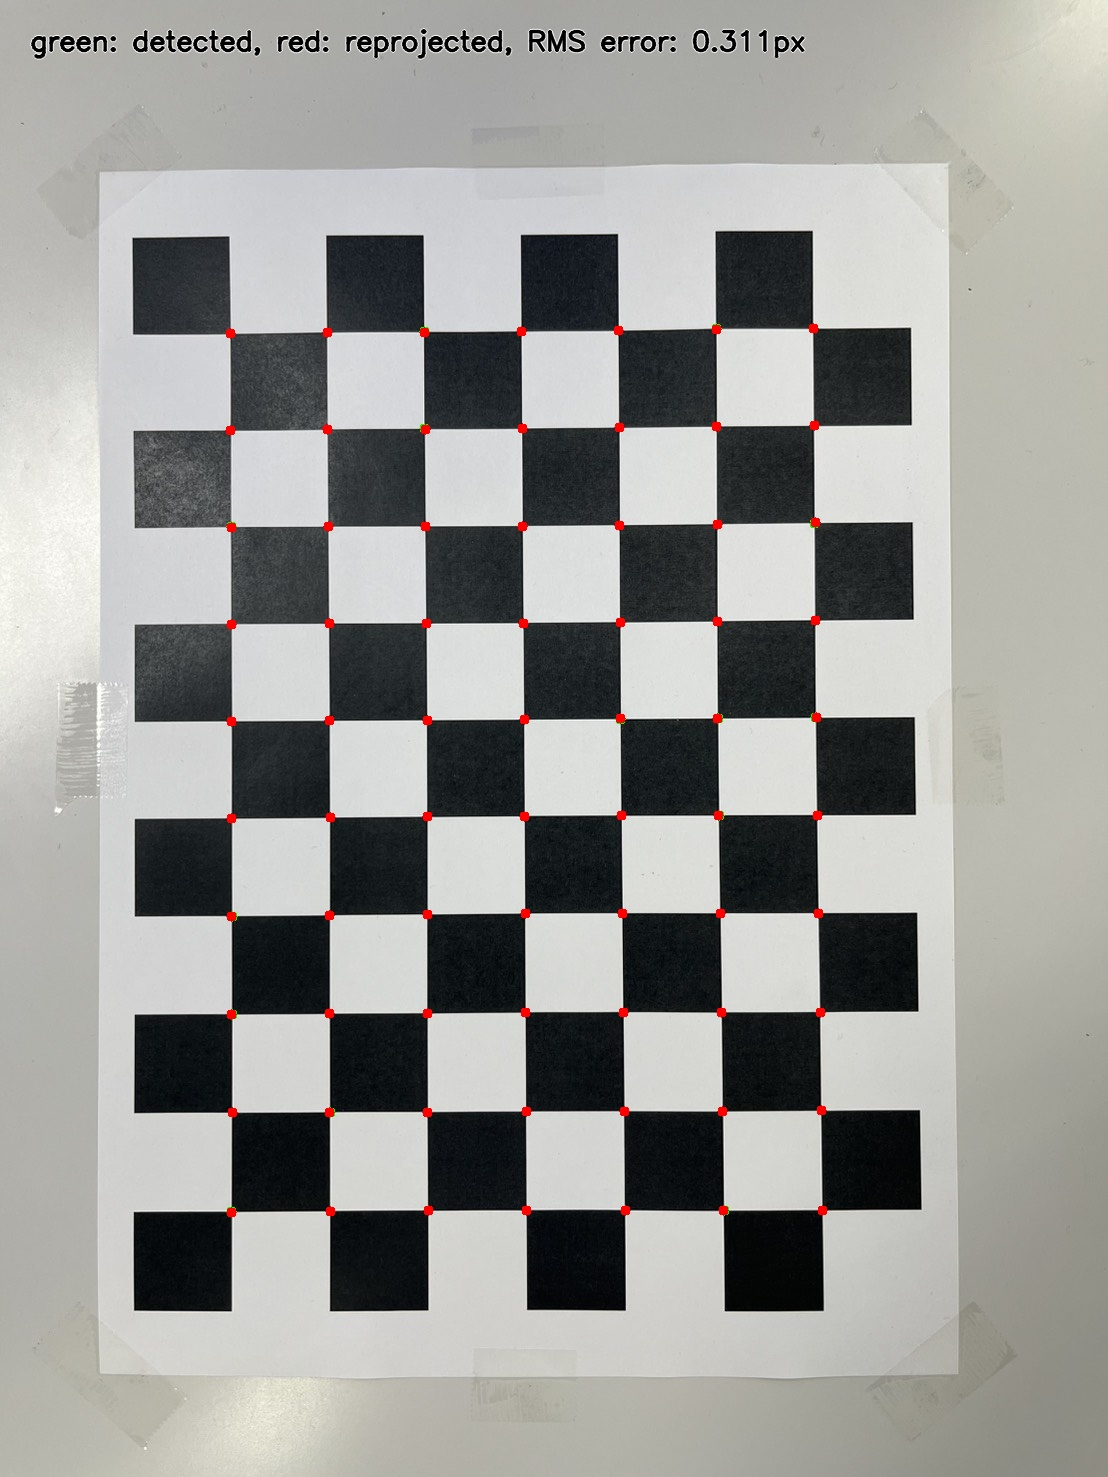
\includegraphics[width=0.46\linewidth]{calibration_outputs/Set_A_3/reprojection_plots/1_reprojection.jpg}
\caption{\texttt{Set\_A\_3} の最小誤差画像（左: \texttt{2.jpg}, 0.112 px）と最大誤差画像（右: \texttt{1.jpg}, 0.311 px）}
\end{figure}

\begin{figure}[H]
\centering

\includegraphics[width=0.46\linewidth]{calibration_outputs/Set_B_7/reprojection_plots/2_reprojection.jpg}
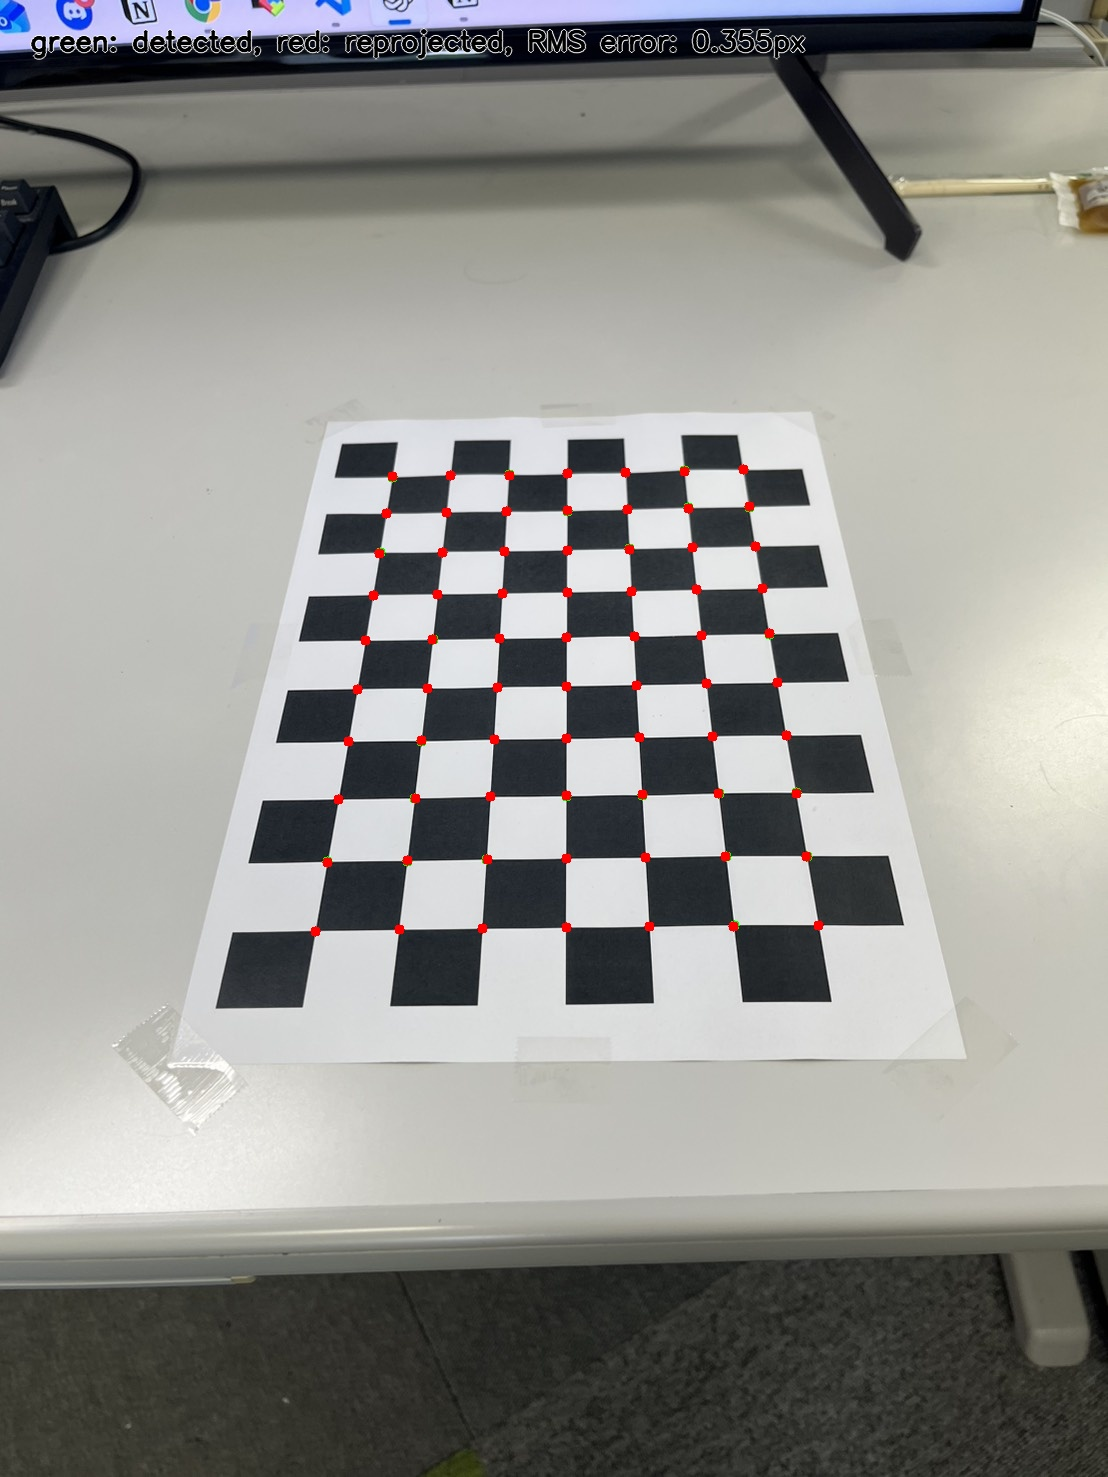
\includegraphics[width=0.46\linewidth]{calibration_outputs/Set_B_7/reprojection_plots/5_reprojection.jpg}
\caption{\texttt{Set\_B\_7} の最小誤差画像（左: \texttt{2.jpg}, 0.107 px）と最大誤差画像（右: \texttt{5.jpg}, 0.355 px）}
\end{figure}

\begin{figure}[H]
\centering

\includegraphics[width=0.46\linewidth]{calibration_outputs/Set_C_11/reprojection_plots/2_reprojection.jpg}
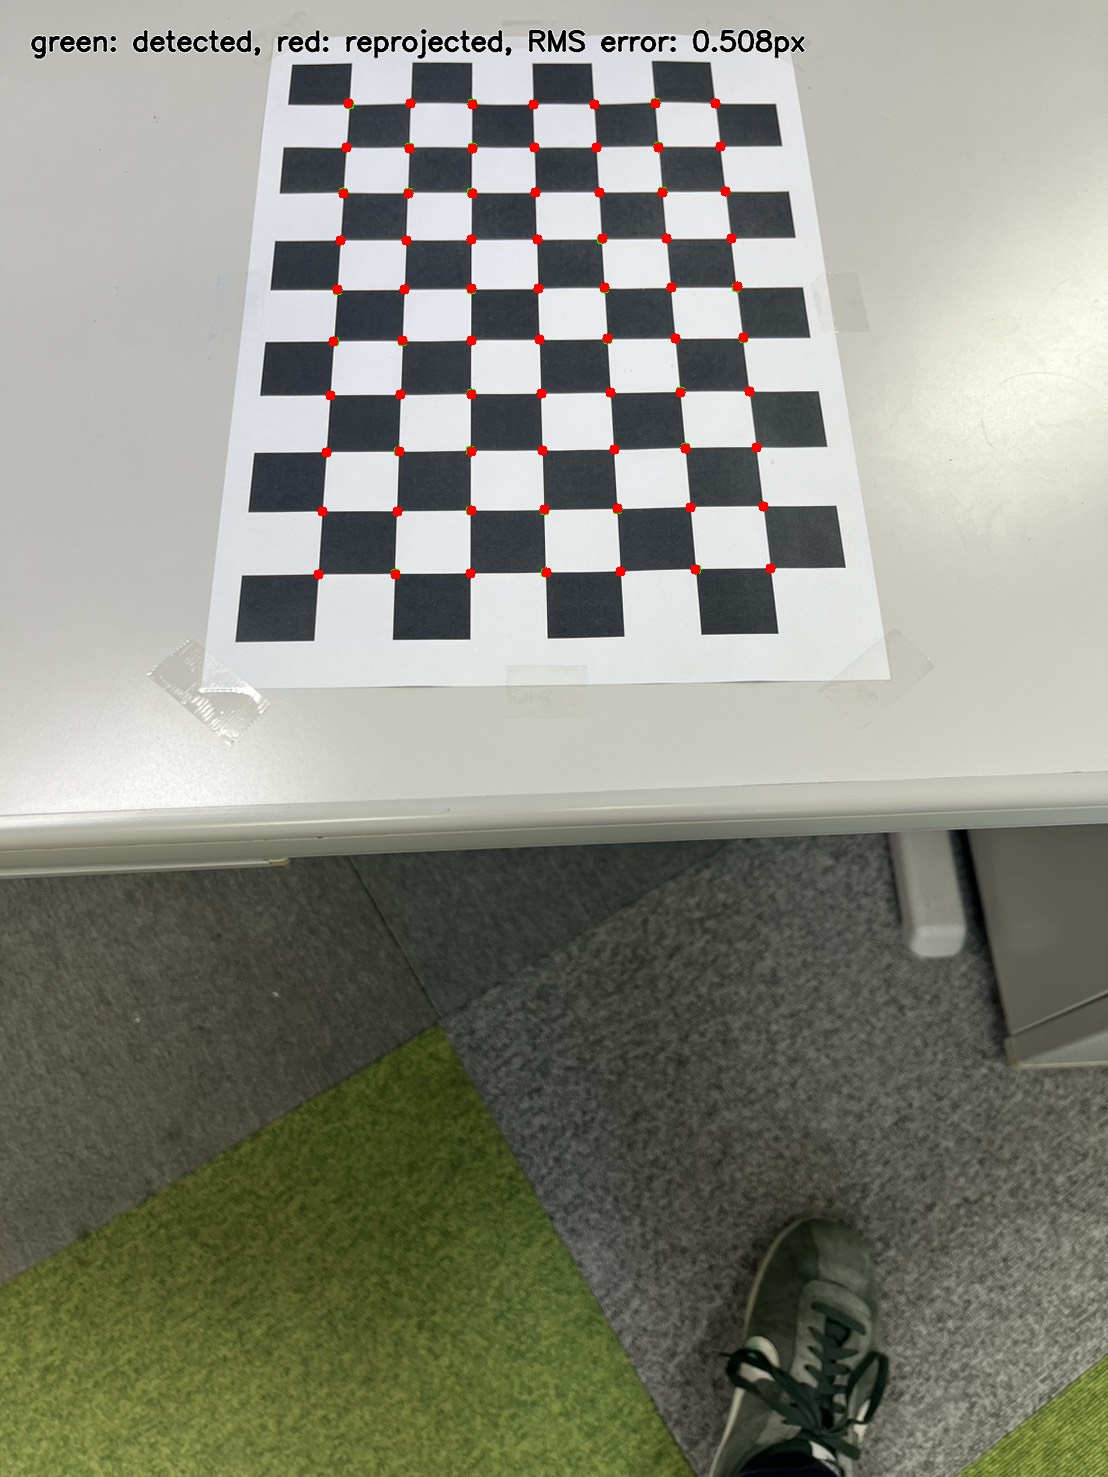
\includegraphics[width=0.46\linewidth]{calibration_outputs/Set_C_11/reprojection_plots/9_reprojection.jpg}
\caption{\texttt{Set\_C\_11} の最小誤差画像（左: \texttt{2.jpg}, 0.128 px）と最大誤差画像（右: \texttt{9.jpg}, 0.508 px）}
\end{figure}

\begin{figure}[H]
\centering

\includegraphics[width=0.46\linewidth]{calibration_outputs/Set_D_15/reprojection_plots/2_reprojection.jpg}
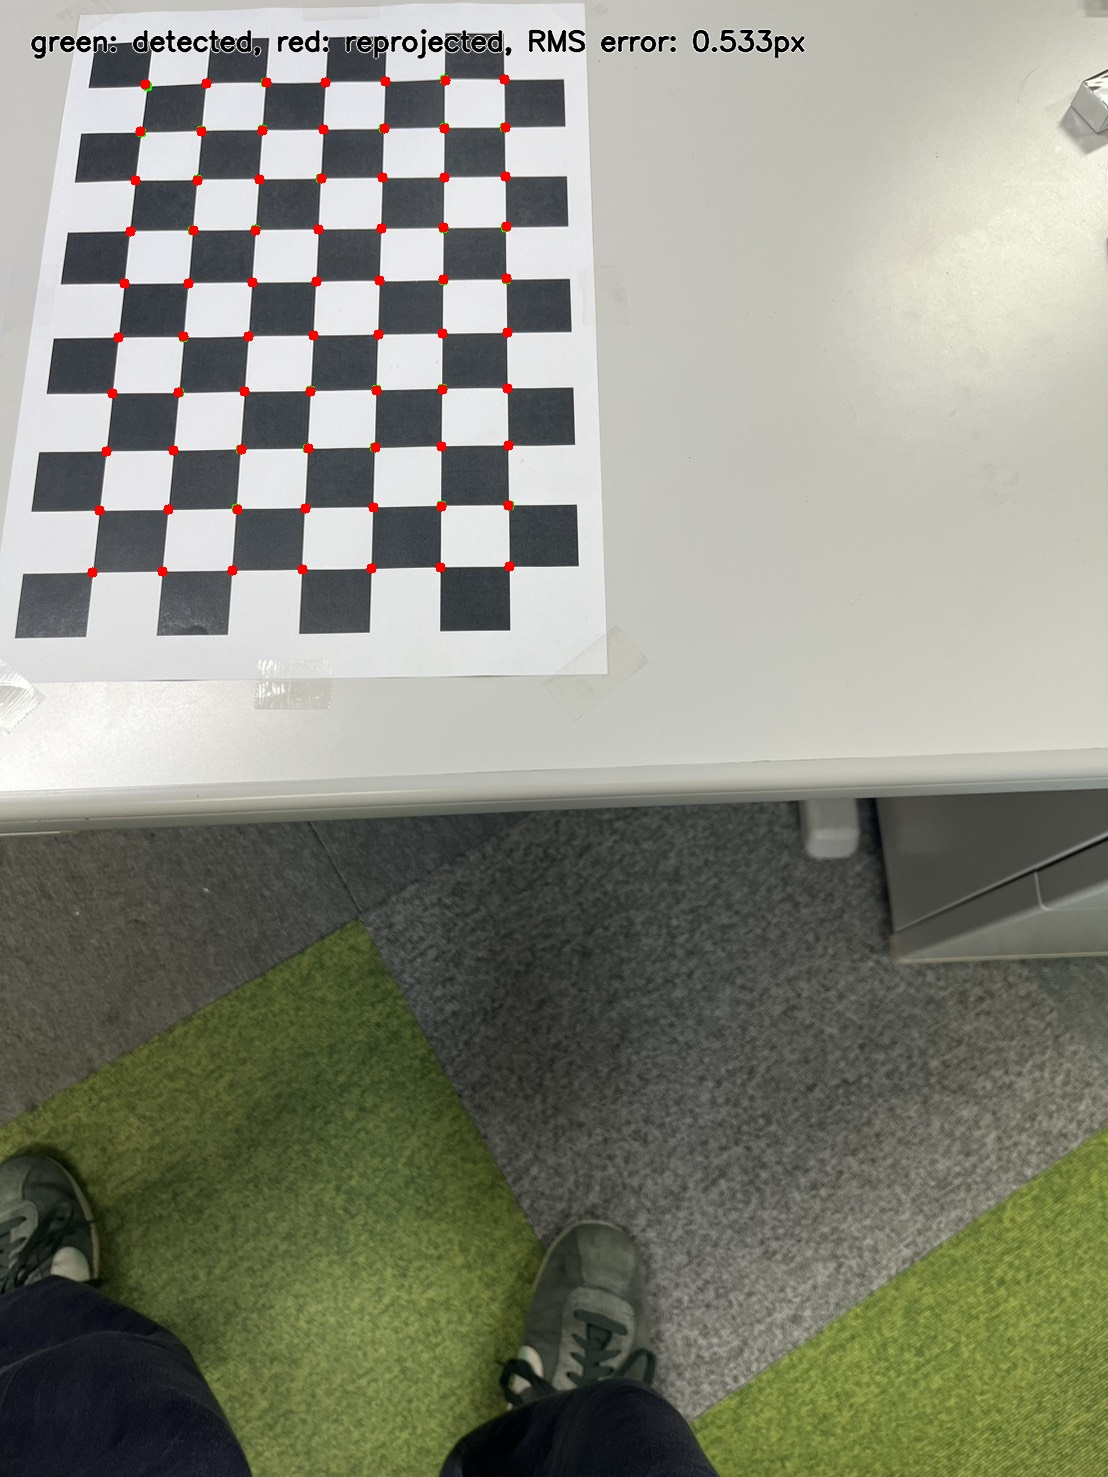
\includegraphics[width=0.46\linewidth]{calibration_outputs/Set_D_15/reprojection_plots/12_reprojection.jpg}
\caption{\texttt{Set\_D\_15} の最小誤差画像（左: \texttt{2.jpg}, 0.192 px）と最大誤差画像（右: \texttt{12.jpg}, 0.533 px）}
\end{figure}

\section*{5. 考察}

まず、3枚のみを用いた \texttt{Set\_A\_3} ではRMS誤差が最も小さくなった。
しかし、この結果だけから \texttt{Set\_A\_3} が最も良いキャリブレーションであるとは
判断できない。RMS誤差は、使用した画像に対して推定されたカメラパラメータが
検出点と再投影点のずれをどの程度小さくできているかを表す値であり、
別の撮影条件での画像に対しても正確であることを直接保証するものではない。
また、チェッカーボードを遠くから撮影すると、画像上でチェッカーボードが小さく写るため、
ピクセル単位の再投影誤差は小さく評価されやすい。
そのため、遠距離、正面、画像中心付近の画像ではRMS誤差が小さく見えやすく、
この点からもRMS誤差だけで精度を判断することは適切ではない。

実際に、\texttt{Set\_A\_3} では焦点距離が
$f_x=1235.763$、$f_y=1234.375$ と推定されており、7枚以上を用いた他のセットと比べて
大きい値になっている。これは、\texttt{Set\_A\_3} に含まれる画像が3枚と少ないことに加え、
チェッカーボードを上から撮影し、対象物が画像中心付近に配置された画像に偏っていたためだと
考えられる。カメラキャリブレーションでは、チェッカーボードをさまざまな角度や位置で
撮影することで、焦点距離、主点、歪み係数を決めるための情報が増える。しかし、
\texttt{Set\_A\_3} のように、チェッカーボードの姿勢変化が小さく、対象物が画像中心付近に
集中している場合、奥行き方向の変化や画像周辺部の歪みに関する情報が不足する。
その結果、内部パラメータを決定するための制約が弱くなり、使用した3枚の画像に対しては
小さい再投影誤差を与えるものの、焦点距離が他のセットと異なる値として推定された
可能性がある。

一方、\texttt{Set\_B\_7}、\texttt{Set\_C\_11}、\texttt{Set\_D\_15} では、
焦点距離はおよそ1140--1146 pxの範囲に収まっており、\texttt{Set\_A\_3} と比べて
大きな変動が見られなかった。このことから、チェッカーボードの位置や
角度の変化を含めることで、内部パラメータを決めるための条件が増えたと考えられる。

歪み係数についても、\texttt{Set\_A\_3} では他のセットと比べて大きな値が推定された。
特に半径方向歪み係数を見ると、\texttt{Set\_A\_3} では
$k_1=0.265$、$k_2=-1.831$、$k_3=4.219$ であったのに対し、
\texttt{Set\_D\_15} では $k_1=0.098$、$k_2=-0.260$、$k_3=0.274$ となった。
この差は、\texttt{Set\_A\_3} ではチェッカーボードが画像中心付近に集中しており、
画像周辺部における歪みを十分に観測できなかったためと考えられる。歪み係数は主に
画像中心から離れた点の変形によって制約されるため、中心付近の画像だけでは焦点距離と
歪み係数の組み合わせに自由度が残りやすい。その結果、\texttt{Set\_A\_3} では
小さいRMS誤差を保ちながらも、歪み係数が大きめに推定された可能性がある。
一方、\texttt{Set\_B\_7} 以降では周辺部や傾いた姿勢の画像が含まれるため、歪みの影響を
反映でき、\texttt{Set\_A\_3} よりも極端でない係数になったと考えられる。
また、接線方向歪みを表す $p_1$、$p_2$ はいずれのセットでも $10^{-4}$ 程度であり、
半径方向歪みに比べて影響は小さいと考えられる。

ただし、画像枚数を増やせばRMS誤差が必ず小さくなるわけではない。
\texttt{Set\_D\_15} では最も多い15枚の画像を用いたにもかかわらず、RMS誤差は
0.425 pxと4つのセットの中で最も大きかった。この理由として、画像数が増えたことで、
チェッカーボードの傾きが大きい画像や、画像周辺部に配置された画像も含まれるようになり、
検出点のわずかな誤差やレンズ歪みの影響がRMS誤差に反映されやすくなったことが
考えられる。つまり、\texttt{Set\_D\_15} のRMS誤差が大きいことは、必ずしも
キャリブレーション精度が悪いことを意味しない。むしろ、多様な条件の画像を含めた結果、
より広い撮影条件に対して妥当なパラメータを推定している可能性がある。

したがって、今回の結果からは、RMS誤差の大小だけでキャリブレーションの良し悪しを
判断するのではなく、推定された内部パラメータの安定性も併せて評価する必要があると
分かる。\texttt{Set\_A\_3} はRMS誤差は小さいが、画像枚数が少なく、さらに上から
撮影した画像や画像中心付近に対象物を配置した画像に偏っている。そのため、撮影条件の
不足による過適合の可能性がある。一方、\texttt{Set\_B\_7} 以降では焦点距離が近い値に
収束しているため、\texttt{Set\_A\_3} よりも信頼性の高いキャリブレーション結果であると
考えられる。

正確なキャリブレーションを行うためには、チェッカーボード全体が画像内に収まり、ぼけや
反射が少ない画像を用いることが重要である。また、正面または上からの画像だけでなく、
上下左右に傾けた画像や、画像中心だけでなく周辺部に配置した画像を含める必要がある。
これにより、焦点距離や歪み係数を推定するための制約が増え、特定の撮影条件に偏りにくい
内部パラメータを得ることができる。

今回の実験では、全てのセットでRMS誤差は1 px未満であり、交点検出も成功している。
そのため、全体としてはキャリブレーションに使用可能な画像品質であったと考えられる。
ただし、最も信頼できる結果を選ぶ際には、RMS誤差が最小である \texttt{Set\_A\_3} ではなく、
画像枚数と撮影条件の多様性があり、かつ内部パラメータが安定している
\texttt{Set\_B\_7} 以降の結果を重視するべきである。

\section*{6. まとめ}

OpenCVを用いて、4種類の画像セットに対してカメラキャリブレーションを行った。
チェッカーボードの1マスは24 mm、交点数は7$\times$10として設定した。
再投影誤差は0.218 pxから0.425 pxの範囲であり、すべて1 px未満であった。
画像枚数が少ない場合は誤差が小さく見えることがあるが、推定値の安定性を考えると、
複数の角度・位置を含む十分な枚数の画像を使うことが重要である。

\clearpage
\section*{付録: 使用したコード}

本課題でカメラキャリブレーションに使用した Python コードを以下に示す。

\lstinputlisting[language=Python]{calibrate_image_sets_opencv.py}

また、使用画像をデータセットごとに一覧表示するために用いたコードを以下に示す。

\lstinputlisting[language=Python]{make_dataset_overviews.py}

\end{document}
